\documentclass[a4paper, 10pt, notitlepage]{article}

\usepackage{moreverb} %para importar codigo

\usepackage{pepotina} %paquete personal para la caratula del DC

\usepackage[spanish,activeacute]{babel}
\usepackage{babel} %paquete de idioma

\usepackage[latin1]{inputenc}

%\usepackage{color}

\usepackage{hyperref}
%\usepackage[all]{hypcap}

\usepackage{caeycaeING}

\usepackage{fancyhdr} %linea sup con comentarios

\usepackage{lscape} %para hoja apaisada

\usepackage{framed} %para crear cajas de texto

\usepackage{lastpage} %ultima pagina

%\usepackage{pstricks}
%\usepackage{uml} %UML

\usepackage{listings}
%\lstset{
%  breaklines=true,                                     % line wrapping on
%  language=ocl,
%  frame=ltrb,
%  framesep=5pt,
%  basicstyle=\normalsize,
%  keywordstyle=\ttfamily\color{OliveGreen},
%  identifierstyle=\ttfamily\color{CadetBlue}\bfseries,
%  commentstyle=\color{Brown},
%  stringstyle=\ttfamily,
%  showstringspaces=ture
%}

\addtolength{\topmargin}{-50pt} 
\addtolength{\textwidth}{105pt}
\addtolength{\textheight}{120pt}
\addtolength{\oddsidemargin}{-50pt}

%\newcommand{\minix}{\textsl{minix }}

%%% Encabezado y pie de p'agina
\pagestyle{fancy}
\fancyhead[LO]{Ingenieria del Software I}
\fancyhead[C]{}
\fancyhead[RO]{P\'agina \thepage\ de \pageref{LastPage}}
\renewcommand{\headrulewidth}{0.4pt}
\fancyfoot{}

\newcommand{\depto}{{\bf DPTO: }}


\def\falta#1{ \begin{framed}	\begin{center} \hspace{1cm} \Large FALTA \normalsize #1 \hspace{1cm} \end{center} \end{framed}}


\def\imagen#1#2#3{\vskip0.5cm
{\large #3}
\begin{center}
\includegraphics[scale=#1]{#2}
\end{center}}


\begin{document}

\universidad{Universidad de Buenos Aires}
\facultad{Facultad de ciencias exactas y naturales}
\departamento{Departamento de Computacion}
\materia{Ingenieria del Software I}
\resumen{Proyecto casino online}
\keys{UML, Objetivos, Agentes, Casos De Uso, Diagrama De Contexto, Modelo Conceptual, OCL, Diagrama de Actividades, FSM}
\titulo{Proyecto: Casino Online}
\subtitulo{Informe 1: Analisis de Requerimientos y especificaci�n}
\grupo{Numero de grupo: 2}
\fecha{1er Cuatrimeste 2008}
\footspace{1cm}
\integrante{Aquino, Isis}{313/05}{isisaquino@yahoo.com.ar}
\integrante{Alvarez, Maria de los Angeles}{264/05}{mdelosaalvarez@hotmail.com}
\integrante{Engler, Christian Alejandro}{314/05}{caeycae@gmail.com}

%caratula
\maketitle{}

\tableofcontents

\newpage

\section{Introducci�n}

\section{Vista Modular}
\label{sec:VistaModular}

Para organizar el dise�o, dividimos el problema en varios problemas independientes con el fin de hacer el dise�o mas flexible y con espectativas de ocultamiento por capas, de modo de que a cada capa se le pudiera cambiar la implementacion.

\imagen{0.70}{img/componentes.png}{Vista Modular}

\newpage
\paragraph{Descripcion de cada uno de los modulos}
\label{sec:DescripcionDeCadaUnoDeLosModulos}

\begin{description}
	\item[Mensajero] El modulo mensajero se ocupa de recibir los mensajes que le envian los clientes al servidor del casino online. Sus obligaciones son ``chequear'' la llegada de un mensaje, empaquetarlo y entregarselo al siguiente modulo.
	\item[Interprete] El modulo interprete se ocupa de tomar un mensaje e intentar trasformarlo a un lenguaje entendible por los servicios del casino, en caso de que el mensaje no corresponda al formato esperado, debera notificar al cliente. Para lograr esta transformacion hace uso del modulo Parser.
	\item[Parser] Este modulo convierte los datos del lenguaje de comunicacion al lenguaje que maneja el casino y viceversa. Esto es para que la eleccion del lenguaje de cada una de estas partes sea independiente y no afecte al resto del sistema.
	\item[Servicios] Este modulo nuclea todos los servicios que presenta el casino. El dise�o del casino esta ocultado detras de este modulo para que la implementacion de estos servicios pueda ser modificada sin grandes efectos colaterales.
	\item[Casino] Aqui esta el casino propiamente dicho, intependiente a toda forma de comunicacion y protocolo. Este modulo se encarga de realizar todo lo especificado en el informe I.
\end{description}
\newpage

\section{Modulos}
\label{sec:Modulos}

\subsection{Mensajero - Interpretador}
\label{sec:MensajeroInterpretador}

Dise�amos un servicio ``core'' de mensajeria para que administre el la recepcion de mensajes independientemente del uso que se le de a ellos.\\
Presentamos aqui un diagrama de secuencia un ejemplo de uso correcto del servicio de mensajeria.
No nos compretemos a que la implementacion del servicio sea ``porArchivos'', pero respetar� el modelo propuesto por la clase abstracta mensajero.
\imagen{0.50}{img/mensajeroSeq.png}{Diagrama de Secuencia: Mensajero}
\newpage

Ahora veamos mas en particular la operacion \textbf{OnMessage}. Esta operacion invoca al listener asociado al mensajero, dicha clase dira al mensajero que operacion realizar en el momento de recibir un mensaje.
\imagen{0.50}{img/onMessageSeq.png}{Diagrama de Secuencia: OnMessage}
\newpage

Para completar la explicacion del dise�o de este modulo necesitamos el diagrama de clases.

\imagen{0.50}{img/mensajeroInterpretador.png}{Diagrama de Clases: Mensajero - Interpretador}
\newpage

\subsection{Interpretador - Parser - Servicios}

No hay mucha complejidadad en estas interacciones y estan suficientemente ilustradas en el diagrama de secuencia anterior. Presentamos el diagrame de clases de los modulos restantes.

\imagen{0.50}{img/interpretadorServicios.png}{Diagrama de Clases: Interpretador - Parser - Servicios}
\newpage

\subsection{Casino}
\newpage

\section{Funcionalidad Casino}
\label{sec:FuncionalidadCasino}

\subsection{Registracion y Ingreso al casino online y modificacion de saldo}

\subsubsection{Registracion}

Segun lo acordado en la especificacion, la registracion de los usuarios se hace por fuera del sistema informatico del casino online.\\
En el momento de abrir el casino el sistema contar� con un archivo XML (en el futuro podria ser de otra manera)
\\
\textbf{Dicho archivo tendr� la siguiente sintaxis:}

\begin{verbatim}
<jugadores>
    <jugador nombre="Nombre" saldo"valor numerico del saldo" vip="true | false">
</jugadores>
\end{verbatim}

\subsubsection{Modificacion de saldo}

Las modificaciones de saldo real solo se pueden realizar mientras el casino permanece cerrado.\\
Mas alla de la operatoria, debar� modificarse el archivo definido en el punto anterior con el monto correspondiente antes de la proxima apertura del casino.

\subsubsection{Ingreso y egreso del casino}

En esta seccion estamos apuntando al ingreso de jugadores al casino (no al ingreso de jugadores observadores, dicha interaccion con el casino esta mostrada en la seccion Invitado)

Presentamos aqui diagramas de secuencia del correcto ingreso al casino online.

\newpage
\imagen{0.5}{img/entrar.png}{Jugador entrando al casino aceptado}

\newpage
\imagen{0.5}{img/salir.png}{Jugador saliendo al casino aceptado}


\newpage
\subsection{Administracion del Casino}

\subsubsection{Apertura del casino}

\begin{verbatim}
<valorFichas>
        <valorFicha valor="" />
</valorFichas>
<probablilidades>
    <jugadaFeliz proba="" montoMinimo="" />
    <jugadaTodosPonen proba="" />
    <jugadaNormal proba=""  />
    <craps>
        <valorDado numero="1" proba="" />
        .
        .
        <valorDado numero="6" proba="" />
    </craps>
    <traga>
        <gordoProgresivo montoMinimo="" descuento=""/>
        <combinaciones>
            <combinacion simbolo1="" simbolo2="" simbolo3="" proba=""/>
        </combinaciones>
    </traga>
</probablilidades>
\end{verbatim}

\falta{TODO lo de apertura del casino}

\subsubsection{Clausura del casino}

\falta{TODO lo de apertura del casino}

\newpage
\subsection{Invitado}

En esta seccion estamos apuntando al ingreso de invitados al casino.

Presentamos aqui diagramas de secuencia del correcto ingreso al casino online.

\imagen{0.5}{img/entrarInvitado.png}{Jugador entrando al casino aceptado}

\newpage
\imagen{0.5}{img/salirInvitado.png}{Jugador saliendo al casino aceptado}

\newpage
\subsection{Modo Dirigido}

\subsubsection{Inicio de Modo Dirigido}

\imagen{0.5}{img/setearMD.png}{Jugador saliendo al casino aceptado}

\newpage
\subsubsection{Seteo de Jugadas Feliz y Todos Ponen}

\imagen{0.5}{img/setearJF.png}{Jugador saliendo al casino aceptado}
\newpage
\imagen{0.5}{img/setearTP.png}{Jugador saliendo al casino aceptado}

\newpage
\subsubsection{Finalizaci�n de Modo Dirigido}

\imagen{0.5}{img/resetearMD.png}{Jugador saliendo al casino aceptado}

\newpage
\subsection{Juego Tragamonedas \label{sjt}}
\subsubsection{Entrar en Tragamonedas}
%\imagen{0.5}{img/setearTP.png}{Jugador saliendo al casino aceptado}
\newpage
%\imagen{0.5}{img/setearTP.png}{Jugador saliendo al casino aceptado}

\newpage
\subsubsection{Apostar en Tragamonedas}
%\imagen{0.5}{img/setearTP.png}{Jugador saliendo al casino aceptado}
\newpage
%\imagen{0.5}{img/setearTP.png}{Jugador saliendo al casino aceptado}

\newpage
\subsubsection{Tirar en Tragamonedas}
%\imagen{0.5}{img/setearTP.png}{Jugador saliendo al casino aceptado}
\newpage
%\imagen{0.5}{img/setearTP.png}{Jugador saliendo al casino aceptado}

\newpage
\subsubsection{Salir en Tragamonedas}
%\imagen{0.5}{img/setearTP.png}{Jugador saliendo al casino aceptado}
\newpage
%\imagen{0.5}{img/setearTP.png}{Jugador saliendo al casino aceptado}

\newpage
\subsection{Juego Craps \label{sjt}}
\subsubsection{Entrar en Craps}
%\imagen{0.5}{img/setearTP.png}{Jugador saliendo al casino aceptado}
\newpage
%\imagen{0.5}{img/setearTP.png}{Jugador saliendo al casino aceptado}

\newpage
\subsubsection{Apostar en Craps}
%\imagen{0.5}{img/setearTP.png}{Jugador saliendo al casino aceptado}

\newpage
\subsubsection{Tirar en Craps}
%\imagen{0.5}{img/setearTP.png}{Jugador saliendo al casino aceptado}

\newpage
\subsubsection{Salir en Craps}
%\imagen{0.5}{img/setearTP.png}{Jugador saliendo al casino aceptado}
\newpage
%\imagen{0.5}{img/setearTP.png}{Jugador saliendo al casino aceptado}

\newpage





%%\section{Escenarios en castellano y Diagramas de secuencias de operaciones mas relevantes}
%%
%%\section{Pseudocodigo de operaciones mas complicadas en lo algoritmico}
%%
%%\section{Justificacion, analisis y explicacion de su dise�o}
%%
%%\section{Trazabilidad completa con informe 1}
%%
%%\section{Conclusiones}

%%%- Introduccion. Cambios con respecto al informe 1.
%%%- .
%%%- Pseudocodigo de operaciones mas complicadas en lo algoritmico.
%%%- Diagrama de clases junto una explicacion en castellano de que hace y para sirve cada clase, y de los aspectos mas interesantes del diagrama. Es buena idea factorizar/separar el/los diagramas en base a algun criterio para mostrarlos con mas claridad. Si su dise�o tiene mas de un paquete seria interesante ver las dependencias entre paquetes...
%%%- Justificacion, analisis y explicacion de su dise�o, utilizando desde principios de dise�o, hasta patterns, pasando por depedencias, acoplamiento y cohesion, hasta mas secuencias de ejemplo para explicar porque su dise�o es bueno y elegante al resolver los problemas que se les presentaron.
%%%- Trazabilidad completa con informe 1. Ademas todo el informe va dirigido al area de sistemas de la empresa de los socios.
%%%- Conclusiones.
%%%
%%%Saludos,
%%%Nicolas.






%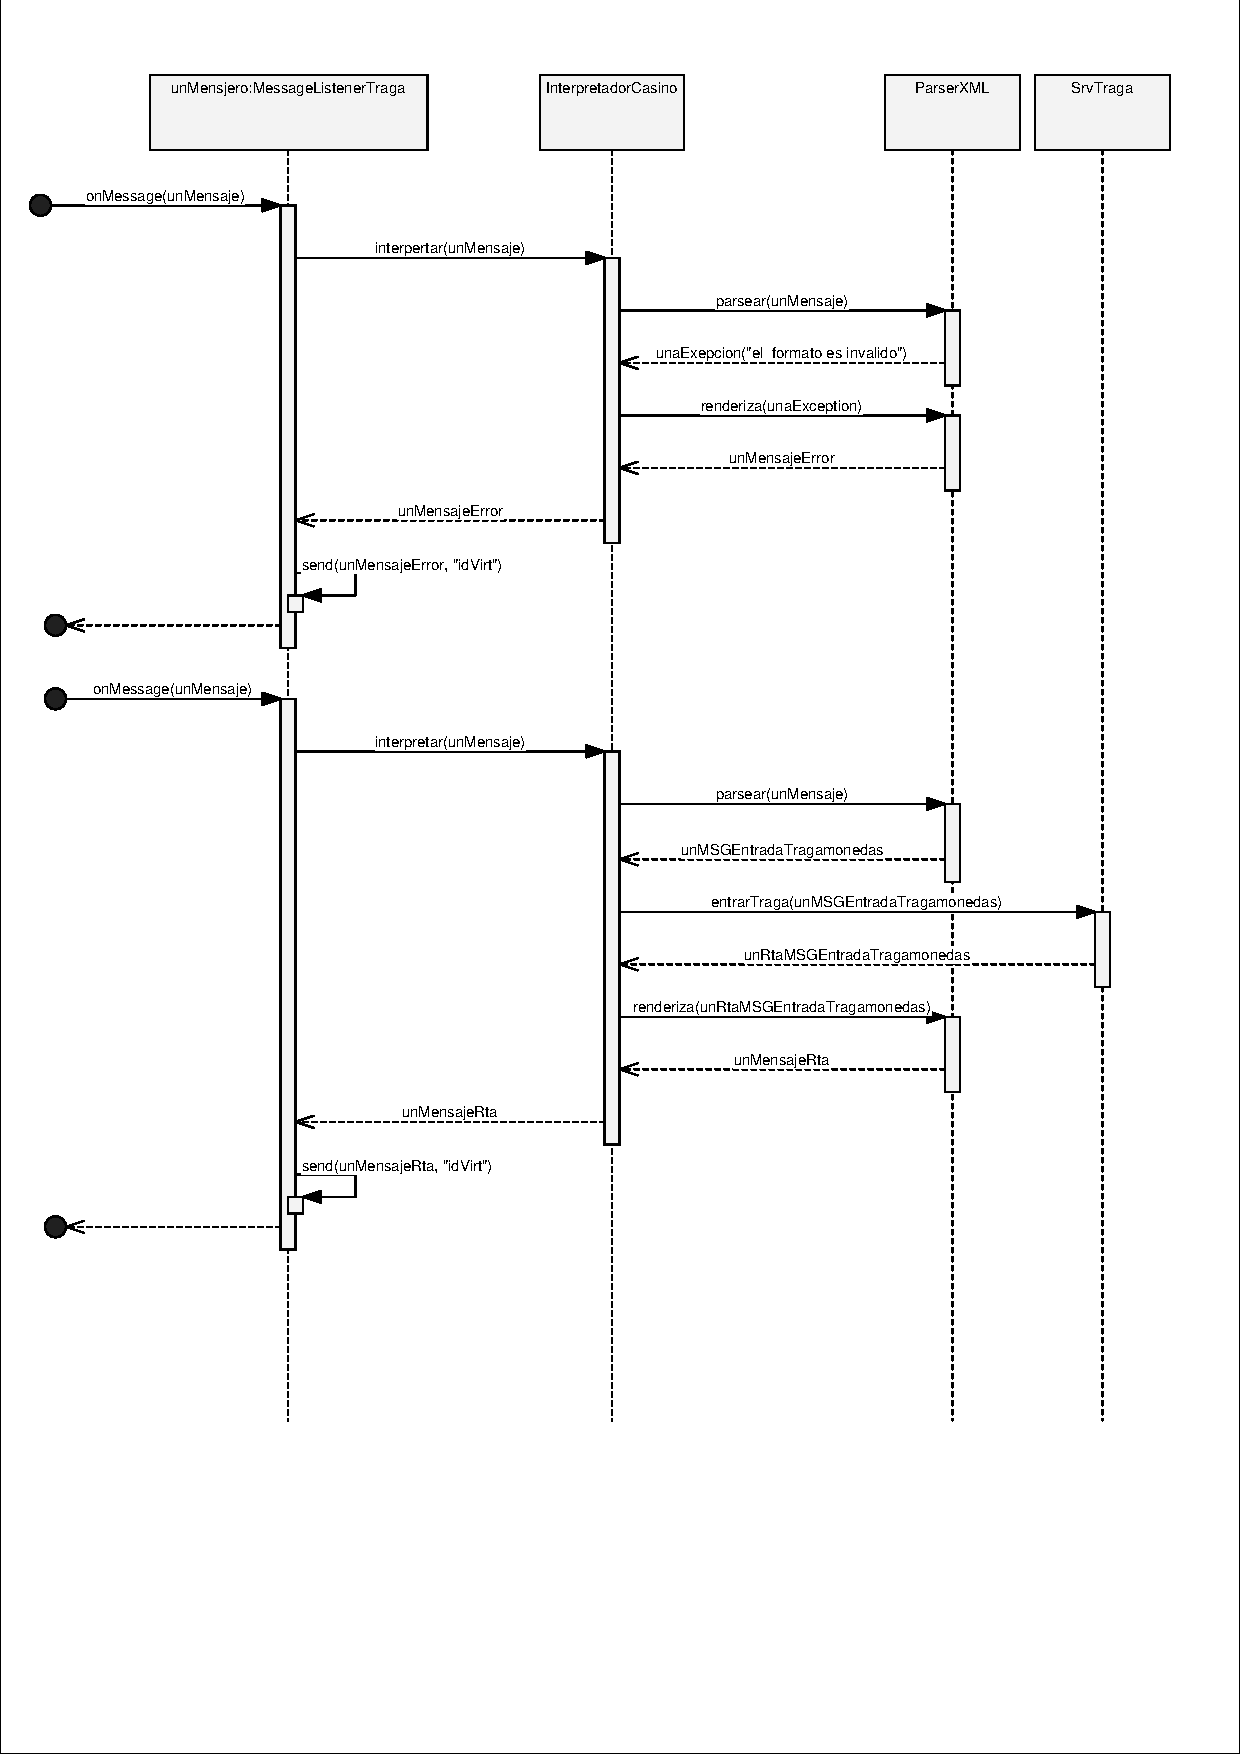
\includegraphics[scale=0.60]{mensajero.pdf}
%,angle=90]
%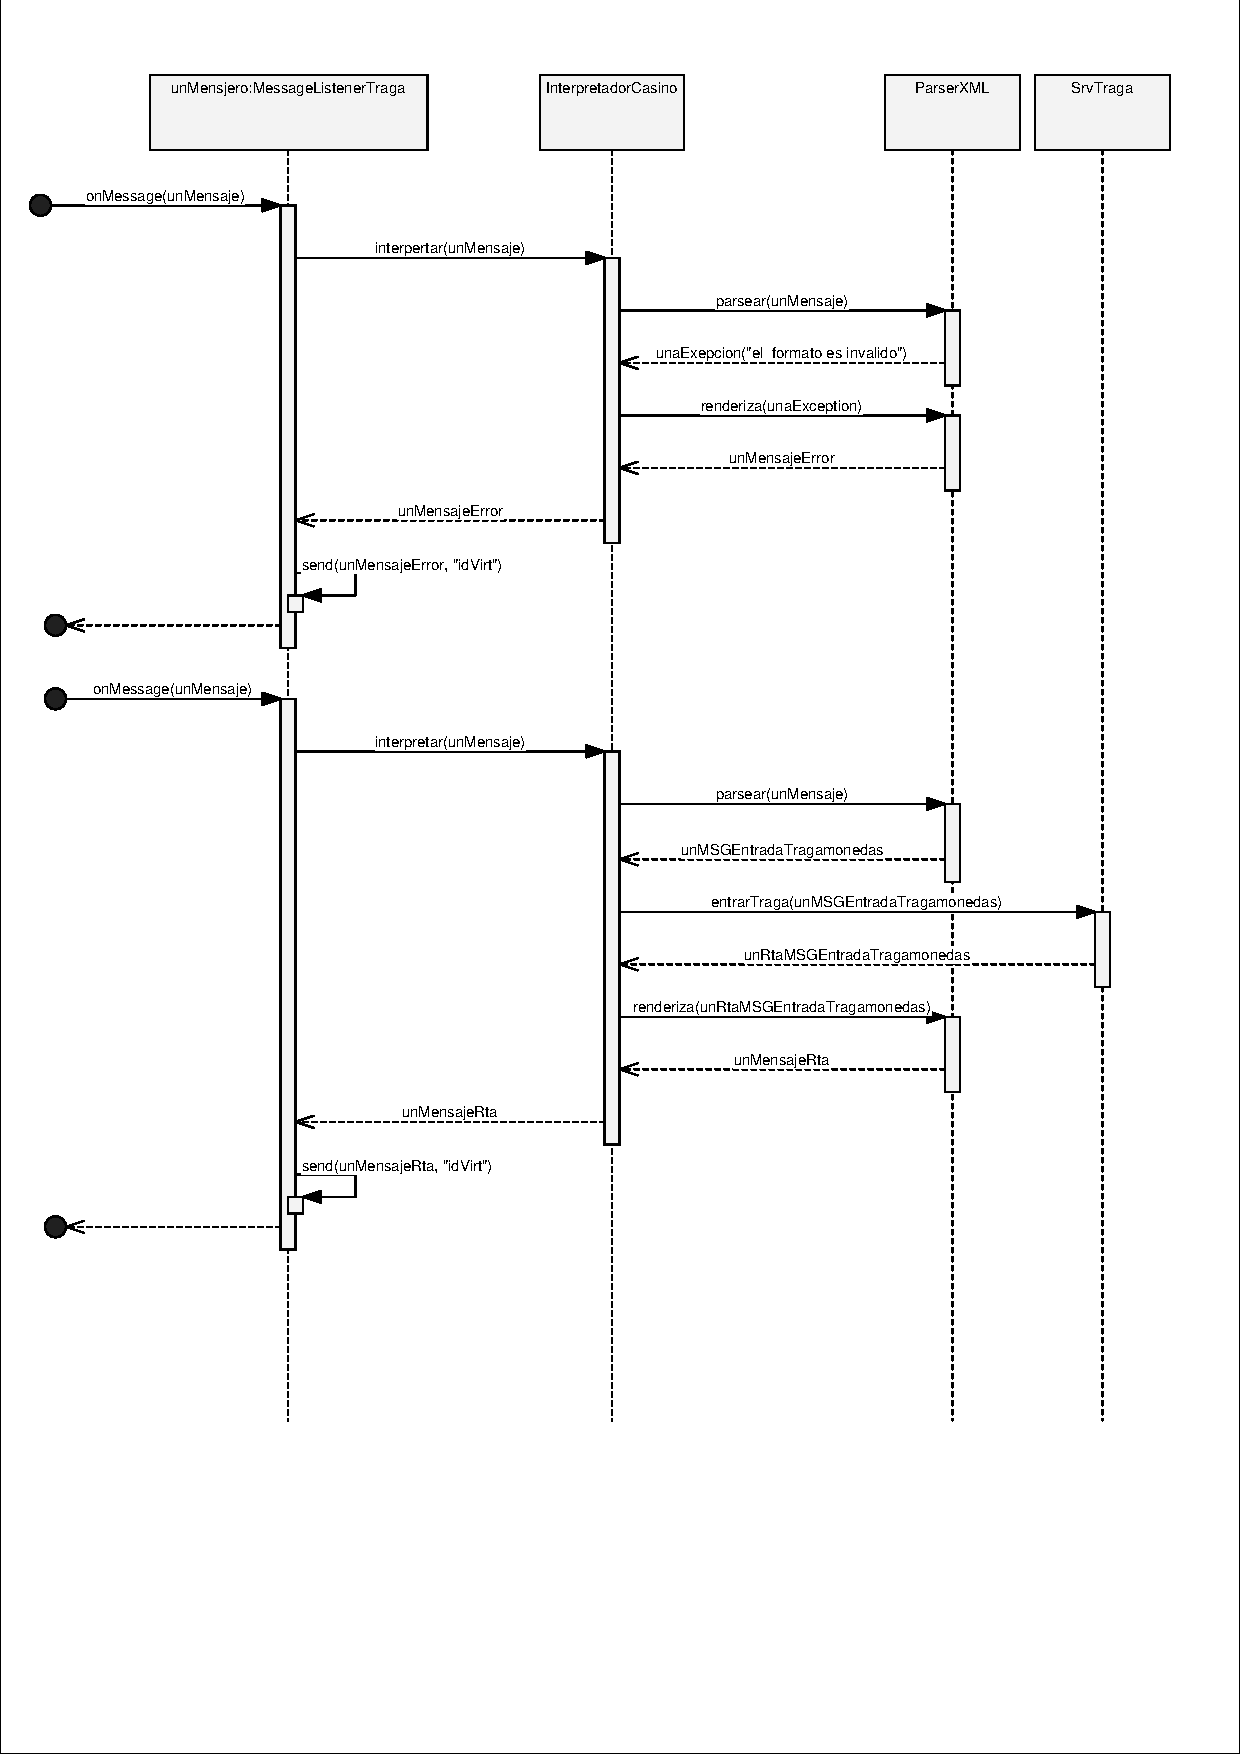
\includegraphics[height=4in,width=6in]{mensajero.pdf}
%  \includegraphics[height=60mm]{myfig.eps}
%  \includegraphics[scale=0.75]{myfig.eps}
%  \includegraphics[angle=45,width=52mm]{myfig.eps}


\end{document}


